\begin{figure}
\centering
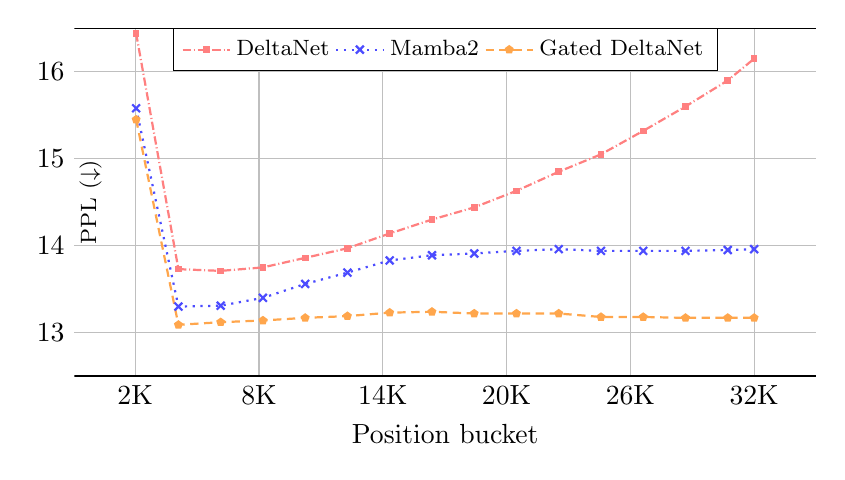
\begin{tikzpicture}
    \begin{axis}[
            width=11cm,
            height=6cm,
            % grid=both,
            ymajorgrids=true,
            xmajorgrids=true,
            tickwidth=0pt,
            tick align=inside,
            axis line style={opacity=0},
            % minor grid style={gray!25},
            % major grid style={gray!25},
            % xlabel={Input Length},
            xtick={2000, 8000, 14000, 20000, 26000, 32000},
            ytick={13, 14, 15, 16},
            xticklabels={2K, 8K, 14K, 20K, 26K, 32K},
            scaled ticks=false,
            ylabel={\footnotesize PPL ($\downarrow$)},
            xlabel={Position bucket},
            ylabel style={font=\footnotesize,at={(0.05,0.5)}},
            ymax=16.5,
            ymin=12.5,
            legend entries={DeltaNet, Mamba2, Gated DeltaNet},
            % legend pos=south east,
            legend style={
                    font=\footnotesize,
                    legend columns=4,
                    at={(0.5,1.)},
                    anchor=north,
                },
            % restrict y to domain=8.6:10,
            % clip=true,
        ]

        % \begin{scope}[on above layer]
        %     \node[anchor=south east, rounded corners=5pt, anchor=west, align=center, draw=gray] (commit) at ($(axis cs: 2048, 10) + (10pt, 0pt)$) {\textcolor{red}{TODO: Something like}\\ Xfmr's PPL blow up!};
        %     \draw[-, thin, shorten <=0pt, shorten >=2.8pt, out=180, in=0, gray] (commit) to ($(axis cs: 2048, 10) + (0pt, 2pt)$);
        % \end{scope}

        \addplot[
            densely dashdotted,
            mark=square*, draw=red!50, thick,
            mark size=0.8pt,
            mark options={fill=red!50, fill opacity=1.0, solid},
            opacity=1.0,
        ] coordinates {
                ( 2048, 16.44)
                ( 4096, 13.73)
                ( 6144, 13.71)
                ( 8192, 13.75)
                (10240, 13.86)
                (12288, 13.97)
                (14336, 14.14)
                (16384, 14.30)
                (18432, 14.44)
                (20480, 14.63)
                (22528, 14.85)
                (24576, 15.05)
                (26624, 15.32)
                (28672, 15.60)
                (30720, 15.90)
                (32000, 16.15)
            };

        \addplot[
            dotted,
            mark=x, draw=blue!70, thick,
            mark size=2pt,
            mark options={
                    % fill=white,
                    fill opacity=0.5,
                    solid},
            opacity=1.0,
        ] coordinates {
                ( 2048, 15.58)
                ( 4096, 13.30)
                ( 6144, 13.31)
                ( 8192, 13.40)
                (10240, 13.56)
                (12288, 13.69)
                (14336, 13.83)
                (16384, 13.89)
                (18432, 13.91)
                (20480, 13.94)
                (22528, 13.96)
                (24576, 13.94)
                (26624, 13.94)
                (28672, 13.94)
                (30720, 13.95)
                (32000, 13.96)
            };

        \addplot[
            densely dashed,
            mark=pentagon*, draw=orange!70, thick,
            mark size=1.2pt,
            mark options={
                    fill=orange!70,
                    fill opacity=1.0, solid
                },
            opacity=1.0,
        ] coordinates {
                ( 2048, 15.45)
                ( 4096, 13.09)
                ( 6144, 13.12)
                ( 8192, 13.14)
                (10240, 13.17)
                (12288, 13.19)
                (14336, 13.23)
                (16384, 13.24)
                (18432, 13.22)
                (20480, 13.22)
                (22528, 13.22)
                (24576, 13.18)
                (26624, 13.18)
                (28672, 13.17)
                (30720, 13.17)
                (32000, 13.17)
            };

        \draw [semithick, black] (axis description cs:0,0) -- (axis description cs:1,0); % This line adds a thick line at y=0
        \draw [semithick, black] (axis description cs:0,1) -- (axis description cs:1,1); % This line adds a thick line at y=1
    \end{axis}


\end{tikzpicture}
\caption{Length extrapolation results in PG19 test set~\citep{pg19}. We split , and only evaluate perplexity within that bucket. }
\label{figure:}
\end{figure}